\section{CHUYỂN ĐỘNG TỔNG HỢP}
\subsection{LÝ THUYẾT TRỌNG TÂM}
\begin{tomtat}
	\subsubsection{Tính tương đối của chuyển động}
	\paragraph{Quỹ đạo có tính tương đối}
		Hình dạng của quỹ đạo của chuyển động trong các hệ quy chiếu khác nhau thì khác nhau.
	\paragraph{Vận tốc có tính tương đối}
	Vận tốc của chuyển động với các hệ quy chiếu khác nhau thì khác nhau. 
	\subsubsection{Hệ quy chiếu đứng yên và hệ quy chiếu chuyển động}
	\begin{dn}
		\begin{itemize}
			\item \textbf{Hệ quy chiếu đứng yên:} là hệ quy chiếu gắn với vật làm mốc được quy ước là đứng yên.\\
			\textit{\textbf{Ví dụ:}} Hệ quy chiếu gắn với sân ga, hệ quy chiếu gắn với bờ sông, \dots
			\item \textbf{Hệ quy chiếu chuyển động:} là hệ quy chiếu gắn với vật làm gốc chuyển động so với hệ quy chiếu đứng yên.\\
			\textit{\textbf{Ví dụ:}} hệ quy chiếu gắn với tàu hoà đang chuyển động, hệ quy chiếu gắn với dòng nước đang trôi, \dots
		\end{itemize}
	\end{dn}
	\subsubsection{Độ dịch chuyển tổng hợp - Vận tốc tổng hợp}
	Quy ước:
	\begin{itemize}
		\item Vật số 1 (người) là vật chuyển động đang được xét.
		\item Vật số 2 (toa tàu) là vật chuyển động được chọn làm gốc của hệ quy chiếu chuyển động.
		\item Vật số 3 (đường ray) là vật đứng yên được chọn làm gốc của hệ quy chiếu đứng yên
	\end{itemize}
	\begin{center}
		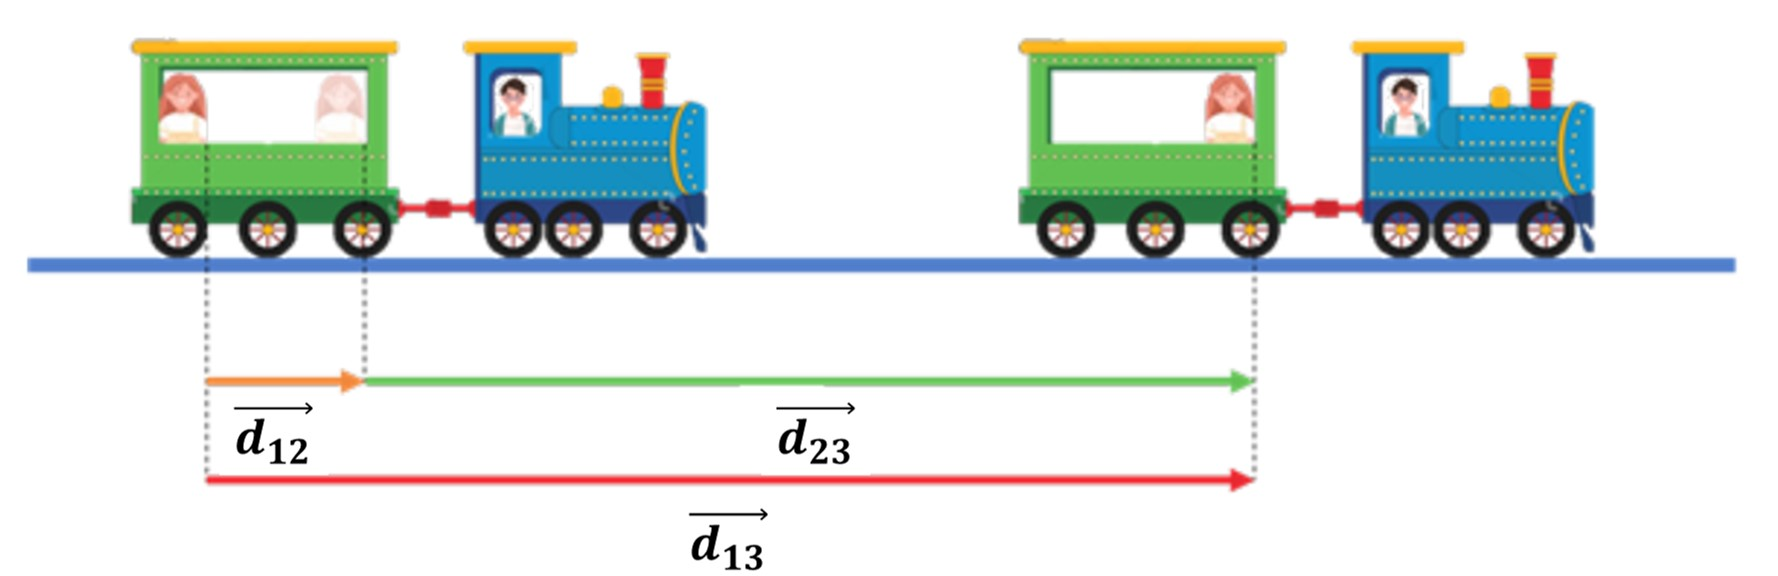
\includegraphics[scale=0.5]{figs/G10Y25B4-1}
	\end{center}
	Khi vật 1 có độ dịch chuyển $\overrightarrow{d_{12}}$ trong hệ quy chiếu chuyển động, đồng thời hệ quy chiếu chuyển động cũng có độ dịch chuyển $\overrightarrow{d_{23}}$ so với hệ quy chiếu đứng yên. Do đó, độ dịch chuyển tổng hợp:
	$$\overrightarrow{d_{13}}=\overrightarrow{d_{12}}+\overrightarrow{d_{23}}$$
	Xét trong khoảng thời gian $\Delta t$ rất bé và kết hợp với định nghĩa của vận tốc:
	$$\dfrac{\overrightarrow{d_{13}}}{\Delta t}=\dfrac{\overrightarrow{d_{12}}}{\Delta t}+\dfrac{\overrightarrow{d_{23}}}{\Delta t}$$
	\begin{noidung}{Công thức cộng vận tốc}
			$$\overrightarrow{v_{13}}=\overrightarrow{v_{12}}+\overrightarrow{v_{23}}$$
		Trong đó:
		\begin{itemize}
			\item $\overrightarrow{v_{13}}$: vận tốc tuyệt đối (vận tốc của vật đối với hệ quy chiếu đứng yên);
			\item $\overrightarrow{v_{12}}$: vận tốc tương đối (vận tốc của vật đối với hệ quy chiếu chuyển động);
			\item $\overrightarrow{v_{23}}$: vận tốc kéo theo (vận tốc của hệ quy chiếu chuyển động đối với hệ quy chiếu đứng yên).
		\end{itemize}
	\end{noidung}

	\begin{center}
		\setlength\arrayrulewidth{1.5pt}
		\begin{tabular}{|M{8.85cm}|M{8.85cm}|}
			\hline
			\rowcolor{violet!30!white}\textbf{Trường hợp 1:} $\overrightarrow{v_{12}}\upuparrows \overrightarrow{v_{23}}$ &\textbf{Trường hợp 2:} $\overrightarrow{v_{12}}\uparrow\downarrow \overrightarrow{v_{23}}$\\
			\hline
				\begin{tikzpicture}
				\coordinate (O) at (0,0);
				\coordinate (B) at (2,0);
				\coordinate (C) at (5,0);
				\coordinate (D) at (2.5,0);
				\coordinate (O1) at ($(O)-(0,1cm)$);
				\coordinate (C1) at ($(C)-(0,1cm)$);
				\coordinate (D1) at ($(D)-(0,1cm)$);
				\draw[-stealth, red, line width=2pt] (O) -- (B);
				\draw[-stealth,blue, line width=2pt] (B) -- (C);
				\draw[-stealth,, line width=2pt] (O1) -- (C1);
				\foreach \i in {O,O1}{
					\filldraw[black] (\i) circle (0.5mm);
				}
				\node[label={[red]90:$\overrightarrow{v_{12}}$}] at (B){};	
				\node[label={[blue]90:$\overrightarrow{v_{23}}$}] at (C){};	
				\node[label=90:$\overrightarrow{v_{13}}$] at (D1){};	
			\end{tikzpicture} & 
			\begin{tikzpicture}
				\coordinate (O) at (0,0);
				\coordinate (B) at (4,0);
				\coordinate (C) at (-2,0);
				\coordinate (D) at (2,0);
				\coordinate (E) at (1,0);
				\coordinate (O1) at ($(O)-(0,1cm)$);
				\coordinate (D1) at ($(D)-(0,1cm)$);
				\coordinate (E1) at ($(E)-(0,1cm)$);
				\draw[-stealth, line width=2pt, red] (O) -- (B);
				\draw[-stealth, line width=2pt, blue] (O) -- (C);
				\draw[-stealth, line width=2pt] (O1) -- (D1);
				\foreach \i in {O,O1}{
					\filldraw[black] (\i) circle (0.5mm);
				}
				\node[label={[red]90:$\overrightarrow{v_{12}}$}] at (B){};	
				\node[label={[blue]90:$\overrightarrow{v_{23}}$}] at (C){};	
				\node[label=90:$\overrightarrow{v_{13}}$] at (E1){};	
			\end{tikzpicture}\\
			$$v_{13}=v_{12}+v_{23}$$ & $$v_{13}=\left|v_{12}-v_{23}\right|$$\\
			\hline
			\rowcolor{violet!30!white}\textbf{Trường hợp 3:} $\overrightarrow{v_{12}} \bot \overrightarrow{v_{23}}$ &  \textbf{Trường hợp 4:} $\left(\overrightarrow{v_{12}},\overrightarrow{v_{23}}\right)=\alpha$\\
			\hline
			\begin{tikzpicture}
				\coordinate (O) at (0,0);
				\coordinate (B) at (4,0);
				\coordinate (C) at (0,3);
				\coordinate (D) at (4,3);
				\coordinate (E) at (1,0);
				\coordinate (O1) at ($(O)-(0,1cm)$);
				\coordinate (D1) at ($(D)-(0,1cm)$);
				\coordinate (E1) at ($(E)-(0,1cm)$);
				\draw[-stealth, line width=2pt, red] (O) -- (B);
				\draw[-stealth, line width=2pt, blue] (O) -- (C);
				\draw[-stealth, line width=2pt] (O) -- (D);
				\draw[dashed] (B) -- (D);
				\draw[dashed] (C) -- (D);
				\foreach \i in {O}{
					\filldraw[black] (\i) circle (0.5mm);
				}
				\tkzMarkRightAngle[draw=black,size=.4](B,O,C);
				\node[label={[red,below right]90:$\overrightarrow{v_{12}}$}] at (B){};	
				\node[label={[blue]90:$\overrightarrow{v_{23}}$}] at (C){};	
				\node[label=90:$\overrightarrow{v_{13}}$] at (D){};	
			\end{tikzpicture} &
			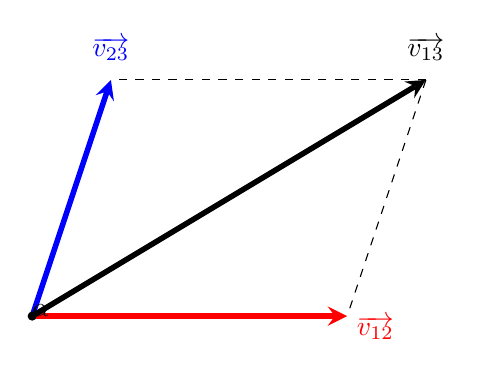
\begin{tikzpicture}
				\coordinate (O) at (0,0);
				\coordinate (B) at (4,0);
				\coordinate (C) at (5,3);
				\coordinate (D) at (1,3);
				\draw[-stealth, line width=2pt, red] (O) -- (B);
				\draw[-stealth, line width=2pt, blue] (O) -- (D);
				\draw[-stealth, line width=2pt] (O) -- (C);
				\draw[dashed] (C) -- (D);
				\draw[dashed] (C) -- (B);
				\foreach \i in {O}{
					\filldraw[black] (\i) circle (0.5mm);
				}
				\node[label={[red,below right]90:$\overrightarrow{v_{12}}$}] at (B){};	
				\node[label={[blue]90:$\overrightarrow{v_{23}}$}] at (D){};	
				\node[label=90:$\overrightarrow{v_{13}}$] at (C){};	
				\tkzMarkAngle[size=0.75cm,color=cyan](B,O,D);
				\tkzLabelAngle[color=black,pos=1.0, above](B,O,D){$\alpha$}
			\end{tikzpicture}\\
				$$v_{13}=\sqrt{v^2_{12}+v^2_{23}}$$& 	$$v_{13}=\sqrt{v^2_{12}+v^2_{23}+2v_{12}\cdot v_{23\cdot}\cos\alpha}$$
				Nếu $v_{12}=v_{23}$ thì $v_{13}=2v_{12}\cdot\cos\dfrac{\alpha}{2}$.\\
				\hline
		\end{tabular}
	\end{center}
\end{tomtat}
\subsection{VÍ DỤ MINH HỌA}
\begin{dang}{Phân biệt vật chuyển động và đứng yên trong các hệ quy chiếu khác nhau}
\end{dang}
\begin{vd}
	Một hành khách ngồi trên toa tàu A, nhìn qua cửa sổ thấy toa tàu B bên cạnh và gạch lát sân ga đều chuyển động như nhau. Nếu lấy vật mốc là nhà ga thì:
	\choice
	{Cả hai tàu đều đứng yên}
	{\True Tàu B đứng yên, tàu A chuyển động}
	{Tàu A đứng yên, tàu B chạy}
	{Cả hai tàu đều chạy}
	\loigiai{
		Khi hành khách ngồi trên toa tàu A, mà thấy toa tàu B bên cạnh và gạch lát sân ga đều chuyển động như nhau thì tàu B và sân ga cùng trạng thái chuyển động so với tàu A.
		
		Nếu lấy vật mốc là nhà ga, gạch lát sân ga đứng yên nên tàu B cũng đứng yên. Sân ga chuyển động so với tàu A đồng nghĩa với tàu A chuyển động so với sân ga.
		
		Vậy trong hệ qui chiếu gắn với sân ga (lấy vật mốc là nhà ga), tàu A chuyển động, tàu B đứng yên.
	}
\end{vd}

\begin{vd}
	Hành khách 1 đứng trên toa tàu a, nhìn qua cửa số toa sang hành khách 2 ở toa bên cạnh b. Hai toa tàu đang đỗ trên hai đường tàu song song với nhau trong sân ga. Bỗng 1 thấy 2 chuyển động về phía sau. Tình huống nào sau đây chắc chắn không xảy ra?
	\choice
	{Cả hai toa tàu cùng chạy về phía trước. Toa a chạy nhanh hơn toa b}
	{\True Cả hai toa tàu cùng chạy về phía trước. Toa b chạy nhanh hơn toa a}
	{Toa tàu a chạy về phía trước. Toa b đứng yên}
	{Toa tàu a đứng yên. Toa tàu b chạy về phía sau}
	\loigiai{
		Nếu cả hai tàu cùng chạy về phía trước, tàu b chạy nhanh hơn thì hành khách trên tàu b sẽ chuyển động vượt lên trước hành khách trên tàu a, tức là hành khách 2 sẽ chuyển động về phía trước so với hành khách 1.
	}
\end{vd}
\begin{dang}{Tính vận tốc tuyệt đối, vận tốc tương đối, vận tốc kéo theo}
	Công thức cộng vận tốc:
	$$\overrightarrow{v_{13}}=\overrightarrow{v_{12}}+\overrightarrow{v_{23}}$$
\end{dang}
% ===============================================================
\begin{vd}
	Một ô tô chạy đều trên một đường thẳng với vận tốc \SI{40}{\kilo\meter/\hour}. Một ô tô B đuổi theo ô tô A với vận tốc \SI{50}{\kilo\meter/\hour}. Xác định vận tốc của:
	\begin{enumerate}[label=\alph*.]
		\item xe ô tô B đối với ô tô A,  
		\item xe ô tô A đối với ô tô B.
	\end{enumerate}
	\loigiai{
		Gọi C là một vật đứng yên trên mặt đất trên mặt đất. Hệ quy chiếu gắn với C là hệ qui chiếu đứng yên. Các giá trị vận tốc mà đề bài cho là vận tốc của xe đối với C. 
		
		Trên hình vẽ, ta thể hiện các vectơ vận tốc của các xe A và B đối với C là các vectơ $\vec{v}_{\text{A,C}}$, $\vec{v}_\text{B,C}$.  
		\begin{center}
			\begin{tikzpicture}
				\coordinate (laxis) at (-2,0);
				\coordinate (C) at (0,0);
				\coordinate (A) at (7,0);
				\coordinate (B) at (1,0);
				\coordinate (va) at ($(A)+(2,0)$);
				\coordinate (vb) at ($(B)+(2.5,0)$);
				\coordinate (raxis) at (10,0);
				\draw[->] (laxis) -- (raxis);
				
				
				\draw[->,ultra thick,blue] (A) -- (va);
				\draw[->,ultra thick,green!60!black] (B) -- (vb);
				\node[below=2mm] at (A) {xe A};
				\node[below=2mm] at (B) {xe B};
				\node[below=2mm] at (C) {C};
				\node[right] at (raxis) {$x$};
				\node[above=1mm] at (va) {$\vec{v}_{\text{A,C}}$};
				\node[above=1mm] at (vb) {$\vec{v}_{\text{B,C}}$};
				\coordinate (va2) at ($(A)-(2,0)$);
				\coordinate (vb2) at ($(B)-(2.5,0)$);
				\filldraw (C) circle (4pt);
				\foreach \i in {B,A}
				{
					\filldraw (\i) circle (4pt);
				}
			\end{tikzpicture}
		\end{center}
		\begin{enumerate}[label=\alph*.]
			\item Vận tốc của ô tô B đối với ô tô A là: 	$$\vec{v}_{\textrm{B,A}}=\vec{v}_{\textrm{B,C}}+\vec{v}_{\textrm{C,A}}==\vec{v}_{\textrm{B,C}}-\vec{v}_{\textrm{A,C}},$$
			Chọn chiều dương là chiều chuyển động của hai ô tô.
			Chiếu lên chiều dương, ta được:
			$$v_{\textrm{B,A}}=v_{\textrm{B,C}}-v_{\textrm{A,C}}= 50\, \textrm{km/h}-40\, \textrm{km/h} = 10\, \textrm{km/h}.$$
			\item Vận tốc của ô tô A đối với ô tô B: 	$$\vec{v}_{\textrm{A,B}}=\vec{v}_{\textrm{A,C}}+\vec{v}_{\textrm{C,B}}=\vec{v}_{\textrm{A,C}}-\vec{v}_{\textrm{B,C}}$$
			Chiếu lên chiều dương, ta được:
			$$v_{\textrm{A,B}}=v_{\textrm{A,C}}-v_{\textrm{B,C}}= 40\, \textrm{km/h}-50\, \textrm{km/h} = -10\, \textrm{km/h}.$$
			
			$\bullet$ \textbf{Lưu ý:} Ta cũng có thể suy ra kết quả này từ kết quả câu \textit{a} bằng:
			$$v_{\textrm{A,B}}=-v_{\textrm{B,A}}=-\SI{10}{\kilo\meter/\hour}.$$
		\end{enumerate}	
	}
\end{vd}
\begin{vd}
	Ô tô A chạy đều trên một đường thẳng với tốc độ $\SI{40}{\kilo\meter/\hour}$. Một ô tô B chạy theo phương vuông góc với ô tô A có tốc độ $\SI{30}{\kilo\meter/\hour}$. Xác định tốc độ của xe ô tô B đối với ô tô A.
	\loigiai{
		Ta kí hiệu A là ô tô A, B là ô tô B, C là đất.
		Vận tốc của ô tô B đối với ô tô A: 	$$\vec{v}_{\textrm{B,A}}=\vec{v}_{\textrm{B,C}}+\vec{v}_{\textrm{C,A}}.$$
		Vectơ $\vec{v}_{\textrm{C,A}}=-\vec{v}_{\textrm{A,C}}$ là vectơ cùng độ lớn nhưng ngược hướng với vectơ $\vec{v}_{\textrm{A,C}}$, được biểu diễn bằng vectơ màu đỏ trong hình.
		\begin{center}
			\begin{tikzpicture}[scale=0.8]
				\coordinate (laxis) at (0,0);
				\coordinate (daxis) at (0,0);
				\coordinate (A) at (2,0);
				\coordinate (B) at (0,1);
				\coordinate (va) at ($(A)+(2,0)$);
				\coordinate (vb) at ($(B)+(0,1.5)$);
				\coordinate (raxis) at (5,0);
				\coordinate (uaxis) at (0,3.5);
				\draw[-] (laxis) -- (raxis);
				\draw[-] (daxis) -- (uaxis);
				\draw[->,ultra thick,blue] (A) -- (va);
				\draw[->,ultra thick,green!60!black] (B) -- (vb);
				\node[above=2mm] at (A) {xe A};
				\node[left=2mm] at (B) {xe B};
				%\node[right] at (raxis) {$x$};
				%\node[above] at (uaxis) {$y$};
				\node[below=1mm] at (va) {$\vec{v}_{\text{A,C}}$};
				\node[right=1mm] at (vb) {$\vec{v}_{\text{B,C}}$};
				\coordinate (va2) at ($(A)-(2,0)$);
				\draw[->,ultra thick,red] (A) -- (va2);
				\node[below=1mm] at (va2) {$\vec{v}_{\text{C,A}}$};
				\foreach \i in {B,A}
				{
					\filldraw (\i) circle (2pt);
				}
				\coordinate (O) at (9,1);
				\coordinate (Ou) at ($(O)+(0,1.5)$);
				\coordinate (Ol) at ($(O)-(2,0)$);
				\coordinate (O2) at ($(O)+(-2,1.5)$);
				\draw[->,ultra thick,green!60!black] (O) -- (Ou);
				\draw[->,ultra thick,red] (O) -- (Ol);
				\draw[dashed] (Ou)--(O2);
				\draw[dashed] (Ol)--(O2);
				\draw[->,ultra thick,violet] (O)--(O2);
				\node[below=1mm] at (Ol) {$\vec{v}_{\text{C,A}}$};
				\node[right=1mm] at (Ou) {$\vec{v}_{\text{B,C}}$};
				\node[above left] at (O2) {$\vec{v}_{\text{B,A}}$};
			\end{tikzpicture}
		\end{center}
		
		Do hai ô tô chuyển động theo hai phương vuông góc nhau nên:
		$$v_{\textrm{B,A}}=\sqrt{v_{\textrm{B,C}}^2+v_{\textrm{C,A}}^2}=\sqrt{(\SI{30}{\kilo\meter/\hour})^2+(\SI{40}{\kilo\meter/\hour})^2}=\SI{50}{\kilo\meter/\hour}.$$
	}
\end{vd}
\begin{dang}{Áp dụng công thức cộng vận tốc, tính vận tốc tương đối cùng phương, cùng chiều hoặc ngược chiều với vận tốc kéo theo}
	Khi thuyền chuyển động xuôi dòng:
	$$v_{\text{xd}}=v_{\text{t}}+v_{\text{n}}.$$
	Khi thuyền chuyển động ngược dòng:
	$$v_{\text{nd}}=v_{\text{t}}-v_{\text{n}}.$$
	\end{dang}
\begin{vd}
	Hai bến sông A và B cách nhau $\SI{11.2}{\kilo\meter}$. Một chiếc ca nô phải mất bao nhiêu thời gian để đi từ A đến B rồi trở lại ngay từ B về A. Biết tốc độ của ca nô so với nước không chảy là $v_1=\SI{15}{\kilo\meter/\hour}$ và tốc độ của nước với bờ sông là $v_2=\SI{1}{\kilo\meter/\hour}$.
	\loigiai{
		Ta gọi $v_{\text{xd}}, v_{\text{nd}}$ lần lượt là tốc độ của thuyền đối với bờ khi nó xuôi dòng và ngược dòng.
		
		Tốc độ của thuyền đối với bờ khi thuyền đi xuôi dòng:
		$$v_{\text{xd}}=v_1+v_2 = \SI{16}{\kilo\meter/\hour}.$$
		Thời gian thuyền đi xuôi dòng khi nó đi từ A đến B:
		$$t_{\text{xd}}=\dfrac{\text{AB}}{v_{\text{xd}}}=\dfrac{\SI{11.2}{\kilo\meter}}{\SI{16}{\kilo\meter/\hour}}=\SI{0.7}{\hour}.$$
		Tốc độ của thuyền đối với bờ khi thuyền đi ngược dòng:
		$$v_{\text{nd}}=v_1-v_2 = \SI{14}{\kilo\meter/\hour}.$$
		Thời gian thuyền đi ngược dòng khi nó đi từ B đến A:
		$$t_{\text{nd}}=\dfrac{\text{AB}}{v_{\text{nd}}}=\dfrac{\SI{11.2}{\kilo\meter}}{\SI{14}{\kilo\meter/\hour}}=\SI{0.8}{\hour}.$$
		Tổng thời gian ca nô đi từ A đến B và từ B về A là:
		$$t= t_{\text{xd}}+ t_{\text{nd}}=\SI{0.7}{\hour}+\SI{0.8}{\hour}=\SI{1.5}{\hour}.$$
	}
\end{vd}

\begin{vd}
	Một chiếc thuyền chạy xuôi dòng sông mất $\SI{2}{\hour}$ để chạy thẳng đều từ bến A ở thượng lưu tới bến B ở hạ lưu và phải mất $\SI{3}{\hour}$ khi chạy ngược lại từ bến B về đến bến A. Cho rằng tốc độ của thuyền đối với nước là $v_1=\SI{30}{\kilo\meter/\hour}$, tốc độ của dòng nước đối với bờ sông là $v_2$. Tính khoảng cách AB và $v_2$.
	\loigiai{
		Ta gọi $v_{\text{xd}}, v_{\text{nd}}$ lần lượt là tốc độ của thuyền khi xuôi dòng và ngược dòng.
		
		Tốc độ của thuyền đối với bờ khi thuyền đi xuôi dòng là:
		$$v_{\text{xd}}=v_1+v_2.$$
		Thời gian thuyền đi xuôi dòng khi nó đi từ A đến B:
		\begin{equation*}
			t_{\text{xd}}=\dfrac{\text{AB}}{v_{\text{xd}}}= \dfrac{\text{AB}}{v_1+v_2}\quad \Rightarrow\quad \text{AB}=(v_1+v_2)t_{\text{xd}}
		\end{equation*}
		Tốc độ của thuyền đối với bờ khi thuyền đi ngược dòng là:
		$$v_{\text{nd}}=v_1-v_2.$$
		Thời gian thuyền đi ngược dòng khi nó đi từ B đến A:
		\begin{equation*}
			t_{\text{nd}}=\dfrac{\text{AB}}{v_{\text{nd}}}= \dfrac{\text{AB}}{v_1-v_2}\quad\Rightarrow\quad \text{AB}=(v_1-v_2)t_\text{nd}.
		\end{equation*}
		Từ hai phương trình trên, ta suy ra tốc độ dòng nước và khoảng cách AB:
		\begin{eqnarray*}
			(v_1+v_2)t_{\text{xd}}&=&(v_1-v_2)t_{\text{nd}}\\
			\quad\Rightarrow\quad	v_2&=&\left(\dfrac{t_\text{nd}-t_\text{xd}}{t_{\text{xd}}+t_\text{nd}}\right)\cdot v_1\\
			&=&\left(\dfrac{\SI{3}{\hour}-\SI{2}{\hour}}{\SI{2}{\hour}+\SI{3}{\hour}}\right)\cdot\SI{30}{\kilo\meter/\hour}\\
			&=&\SI{6}{\kilo\meter/\hour},\\
			\quad\Rightarrow\quad \text{AB}&=&(v_1+v_2)t_\text{xd}\\
			&=&(\SI{30}{\kilo\meter/\hour}+\SI{6}{\kilo\meter/\hour})\cdot\SI{2}{\hour}\\
			&=&\SI{72}{\kilo\meter}.
		\end{eqnarray*}
	}
\end{vd}
\subsection{TRẮC NGHIỆM NHIỀU PHƯƠNG ÁN LỰA CHỌN}
\setcounter{ex}{0}
\Opensolutionfile{ans}[ans/G10Y25B4-TN]
\begin{ex}
	Một hành khách ngồi trong xe A, nhìn qua cửa sổ thấy xe B bên cạnh và sân ga đều chuyển động như nhau. Như vậy
	\choice
	{xe A đứng yên, xe B chuyển động}
	{\True xe A chạy, xe B đứng yên}
	{xe A và xe B chạy cùng chiều}
	{xe A và xe B chạy ngược chiều}
	\loigiai{
	}
\end{ex}
\begin{ex}
	Chọn phát biểu \textbf{sai}:
	\choice
	{Vận tốc của chất điểm phụ thuộc vào hệ qui chiếu}
	{Trong các hệ qui chiếu khác nhau thì vị trí của cùng một vật là khác nhau}
	{\True Khoảng cách giữa hai điểm trong không gian là tương đối}
	{Tọa độ của một chất điểm phụ thuộc hệ qui chiếu}
	\loigiai{
		Khoảng cách giữa hai điểm trong không gian không phụ thuộc vào hệ quy chiếu.
	}
\end{ex}
\begin{ex}
	Chọn câu đúng, đứng ở Trái Đất ta sẽ thấy:
	\choice
	{\True Trái Đất đứng yên, Mặt Trời và Mặt Trăng quay quanh Trái Đất}
	{Mặt Trời đứng yên, Trái Đất quay quanh Mặt Trời, Mặt trăng quay quanh Trái đất}
	{Mặt Trời đứng yên, Trái Đất và Mặt Trăng quay quanh Mặt Trời}
	{Mặt Trời và mặt đất đứng yên, Mặt Trăng quay quanh Trái Đất}
	\loigiai{
	}
\end{ex}
\begin{ex}
	Một hành khách ngồi trong toa tàu H, nhìn qua cửa sổ thấy toa tàu N bên cạnh và gạch lát sân ga đều chuyển động như nhau. Hỏi toa tàu nào chạy?
	\choice
	{Tàu N chạy tàu H đứng yên}
	{Cả 2 tàu đều chạy}
	{\True Tàu H chạy tàu N đứng yên}
	{Cả 2 tàu đều đứng yên}
	\loigiai{
	}
\end{ex}

% ===================================================================
\begin{ex}
	Một người đi xe máy từ nhà đến bến xe bus cách nhà $\SI{6}{\kilo\meter}$ về phía Đông. Người đó tiếp tục lên xe bus đi tiếp $\SI{6}{\kilo\meter}$ về phía Bắc. Độ dịch chuyển tổng hợp của người này là	
	\choice
	{$\SI{12}{\kilo\meter}$}
	{$\SI{6}{\kilo\meter}$}
	{\True $\xsi{6\sqrt{2}}{\kilo\meter}$}
	{$\SI{72}{\kilo\meter}$}
	\loigiai{}
\end{ex}
% ===================================================================
\begin{ex}
	Gọi $\vec{v}_{12}$ là vận tốc của vật (1) so với vật (2), $\vec{v}_{23}$ là vận tốc của vật (2) so với vật (3), $\vec{v}_{13}$ là vận tốc của vật (1) so với vật (3). Hệ thức đúng là
	\choice
	{$\vec{v}_{13}=\vec{v}_{12}-\vec{v}_{23}$}
	{$\vec{v}_{13}=\vec{v}_{12}+2\vec{v}_{23}$}
	{\True $\vec{v}_{13}=\vec{v}_{12}+\vec{v}_{23}$}
	{$\vec{v}_{13}=2\vec{v}_{12}+\vec{v}_{23}$}
	\loigiai{}
\end{ex}
\begin{ex}
	Một vật tham gia đồng thời hai chuyển động theo hai phương khác nhau và mỗi phương có tốc độ tương ứng là $v_1$ và $v_2$ so với vật làm mốc. Gọi $v$ là tốc độ tổng hợp của vật so với vận làm mốc. Khi đó
	\choice
	{$v = v_1 + v_2$}
	{$v = |v_1 - v_2|$}
	{$v = \sqrt{v_1^2 + v_2^2}$}
	{\True $|v_1 - v_2| \le v \le v_1 + v_2$}
	\loigiai{}
\end{ex}

\begin{ex}
	Ở một dòng sông, nước đang chảy với tốc độ $v$ so với bờ. Để một con thuyền có thể đứng yên so với bờ thì thuyền cần chuyển động
	\choice
	{\True Với tốc độ $v$ so với nước và ngược chiều dòng nước}
	{Với tốc độ $v$ so với nước và cùng chiều dòng nước}
	{Với tốc độ $v$ so với bờ và ngược chiều dòng nước}
	{Với tốc độ $v$ so với bờ và cùng chiều dòng nước}
	\loigiai{}
\end{ex}

\begin{ex}
	Tốc kế của một ô tô đang chạy chỉ \SI{70}{\kilo\meter/\hour} tại thời điểm $t$. Để kiểm tra xem đồng hồ tốc kế đó chỉ có đúng không, người lái xe giữ nguyên tốc độ, một người hành khách trên xe nhìn đồng hồ và thấy xe chạy qua hai cột cây số bên đường cách nhau \SI{1}{\kilo\meter} trong thời gian \SI{1}{\minute}. Số chỉ của tốc kế
	\choice
	{bằng tốc độ của xe}
	{nhỏ hơn tốc độ của xe}
	{\True lớn hơn tốc độ của xe}
	{bằng hoặc nhỏ hơn tốc độ của xe}
	\loigiai{}
\end{ex}

\begin{ex}
	Ôtô A và ôtô B chạy cùng chiều trên một đoạn đường với tốc độ là \SI{60}{\kilo\meter/\hour} và \SI{50}{\kilo\meter/\hour}. Vận tốc của ôtô A so với ôtô B bằng
	\choice
	{\SI{110}{\kilo\meter/\hour}}
	{\SI{30}{\kilo\meter/\hour}}
	{\True \SI{10}{\kilo\meter/\hour}}
	{\SI{-10}{\kilo\meter/\hour}}
	\loigiai{}
\end{ex}

\begin{ex}
	Một đoàn tàu đang chuyển động đều với tốc độ \SI{10}{\meter/\second}. Trên tàu có một người soát vé đang đi về phía đuôi tàu với tốc độ \SI{1}{\meter/\second} để ổn định khách trong toa tàu. Một học sinh đứng bên đường sẽ thấy người soát vé di chuyển với tốc độ là
	\choice
	{\SI{8}{\meter/\second}}
	{\True \SI{9}{\meter/\second}}
	{\SI{10}{\meter/\second}}
	{\SI{11}{\meter/\second}}
	\loigiai{}
\end{ex}

\begin{ex}
	Bệnh viện Đại học Y Dược có một thang cuốn đặt dọc theo thang bộ có chiều dài $\ell$ giúp người đi nhanh. Nam đi hết thang bộ thì mất \SI{150}{\second}. An đứng yên trên thang cuốn thì hết \SI{70}{\second}. Lan đi dọc theo thang cuốn. Biết Nam và Lan đi thẳng đều với cùng tốc độ. Thời gian Lan đi hết thang cuốn là
	\choice
	{\SI{58}{\second}}
	{\True \SI{48}{\second}}
	{\SI{70}{\second}}
	{\SI{80}{\second}}
	\loigiai{}
\end{ex}

\begin{ex}
	Biết vận tốc của ca nô so với mặt nước đứng yên là $\SI{10}{\meter/\second}$. Vận tốc của dòng nước là $\SI{4}{\meter/\second}$. Vận tốc của ca nô khi đi xuôi dòng là
	\choice
	{\True $\SI{14}{\meter/\second}$}
	{$\SI{9}{\meter/\second}$}
	{$\SI{6}{\meter/\second}$}
	{$\SI{5}{\meter/\second}$}
	\loigiai{
	}
\end{ex}
\begin{ex}
	Hai ô tô A và B chạy cùng chiều trên cùng một đoạn đường với vận tốc $\SI{70}{\kilo\meter/\hour}$ và $\SI{65}{\kilo\meter/\hour}$. Vận tốc của ô tô A so với ô tô B bằng
	\choice
	{$\SI{30}{\kilo\meter/\hour}$}
	{\True $\SI{5}{\kilo\meter/\hour}$}
	{$\SI{135}{\kilo\meter/\hour}$}
	{$\SI{65}{\kilo\meter/\hour}$}
	\loigiai{
	}
\end{ex}
\begin{ex}
	A ngồi trên một toa tàu chuyển động với vận tốc $\SI{15}{\kilo\meter/\hour}$ đang rời ga. B ngồi trên một toa tàu khác chuyển động với vận tốc $\SI{10}{\kilo\meter/\hour}$ đang đi ngược chiều vào ga. Hai đường tàu song song với nhau. Chọn chiều dương là chiều chuyển động của đoàn tàu mà A ngồi. Tính vận tốc của B đối với A.
	\choice
	{$\SI{-5}{\kilo\meter/\hour}$}
	{$\SI{5}{\kilo\meter/\hour}$}
	{$\SI{25}{\kilo\meter/\hour}$}
	{\True $\SI{-25}{\kilo\meter/\hour}$}
	\loigiai{
		Chọn chiều dương là chiều chuyển động của tàu A.
		
		$\vec{v_\text{AD}}$ là vận tốc của tàu A đối với đất;
		
		$\vec{v_\text{BD}}$ là vận tốc của tàu B đối với đất;
		
		$\vec{v_\text{BA}}$ là vận tốc của tàu B đối với tàu A.
		
		Theo công thức cộng vận tốc:
		$$\vec{v_\text{BD}} = \vec{v_\text{BA}}+\vec{v_\text{AD}} \Rightarrow \vec{v_\text{BA}} = \vec{v_\text{BD}} - \vec{v_\text{AD}}=\vec{v_\text{BD}} + \vec{-v_\text{AD}}$$
		
		Chiếu lên chiều chuyển động của tàu A:
		$$v_\text{AB} = -v_\text{BD} - v_\text{AD} = \SI{-10}{\kilo\meter/\hour}-\SI{15}{\kilo\meter/\hour} = \SI{-25}{\kilo\meter/\hour}$$
		
		Vận tốc của tàu B đối với tàu A có độ lớn $\SI{25}{\kilo\meter/\hour}$ và ngược chiều so với chiều chuyển động của tàu A.
	}
\end{ex}
\begin{ex}
	Hai bến sông A và B cùng nằm trên một bờ sông, cách nhau $\SI{18}{\kilo\meter}$. Cho biết độ lớn vận tốc của ca nô đối với nước là $u =\SI{16.2}{\kilo\meter/\hour}$ và độ lớn vận tốc của nước đối với bờ sông là $v=\SI{5.4}{\kilo\meter/\hour}$. Thời gian để ca nô chạy xuôi dòng từ A đến B rồi lại chạy ngược dòng trở về A là
	\choice
	{1 giờ 40 phút}
	{1 giờ 20 phút}
	{\True 2 giờ 30 phút}
	{2 giờ 10 phút}
	\loigiai{
		Thời gian ca nô chạy xuôi dòng từ A đến B rồi chạy ngược lại trở về A:
		$$t=\dfrac{s}{u+v}+\dfrac{s}{u-v}=\dfrac{\SI{18}{\kilo\meter}}{\SI{16.2}{\kilo\meter/\hour}+\SI{5.4}{\kilo\meter/\hour}}+\dfrac{\SI{18}{\kilo\meter}}{\SI{16.2}{\kilo\meter/\hour}-\SI{5.4}{\kilo\meter/\hour}}=\dfrac{\SI{18}{\kilo\meter}}{\SI{21.6}{\kilo\meter/\hour}}+\dfrac{\SI{18}{\kilo\meter}}{\SI{10.8}{\kilo\meter/\hour}}=\SI{0.833}{\hour}+\SI{1.667}{\hour}=\SI{2.5}{\hour}.$$
	}
\end{ex}
\begin{ex}
	Ô tô A chạy thẳng về hướng Tây với độ lớn vận tốc $\SI{40}{\kilo\meter/\hour}$. Ô tô B chạy thẳng về hướng Bắc với độ lớn vận tốc $\SI{60}{\kilo\meter/\hour}$. Độ lớn vận tốc của ô tô B so với người ngồi trên ô tô A gần giá trị nào nhất sau đây?
	\choice
	{$\SI{85}{\kilo\meter/\hour}$}
	{$\SI{90}{\kilo\meter/\hour}$}
	{$\SI{65}{\kilo\meter/\hour}$}
	{\True $\SI{75}{\kilo\meter/\hour}$}
	\loigiai{
		Vận tốc của ô tô B đới với người ngồi trên ô tô A:
		$$\vec{v_{BA}}=\vec{v_{BD}}-\vec{v_{AD}}$$
		Vì $\vec{v_{BD}}\perp \vec{v_{AD}}$ nên
		$$v_{BA}=\sqrt{v^2_{BD}+v^2_{AD}}=\sqrt{(\SI{60}{\kilo\meter/\hour})^2+(\SI{40}{\kilo\meter/\hour})^2}=\sqrt{3600+1600}=\sqrt{5200}\approx\SI{72.1}{\kilo\meter/\hour}.$$
	}
\end{ex}

% ===================================================================
\begin{ex}
	Một chiếc xuồng đi xuôi dòng nước từ A đến B mất 4 giờ, còn nếu đi ngược dòng nước từ B đến A mất 5 giờ. Biết vận tốc của dòng nước so với bờ sông là $\SI{4}{\kilo\meter/\hour}$. Quãng đường AB là
	\choice
	{\True $\SI{160}{\kilo\meter}$}
	{$\SI{120}{\kilo\meter}$}
	{$\SI{130}{\kilo\meter}$}
	{$\SI{150}{\kilo\meter}$}
	\loigiai{}
\end{ex}

\begin{ex}
	Một người lái xuồng máy cho xuồng chạy ngang con sông rộng $\SI{240}{\meter}$. Mũi xuồng luôn luôn vuông góc với bờ sông, nhưng do nước chảy nên xuồng sang đến bờ bên kia tại một điểm cách bến dự định $\SI{180}{\meter}$ về phía hạ lưu và xuồng đi hết $\SI{1}{\minute}$. Độ lớn vận tốc của xuồng so với bờ là
	\choice
	{$\SI{8}{\meter/\second}$}
	{$\SI{9}{\meter/\second}$}
	{$\SI{6}{\meter/\second}$}
	{\True $\SI{5}{\meter/\second}$}
	\loigiai{
		Độ dịch chuyển của xuồng so với vị trí ban đầu:
		$$d=\sqrt{(\SI{240}{\meter})^2+(\SI{180}{\meter})^2}=\sqrt{57600+32400}=\sqrt{90000}=\SI{300}{\meter}.$$
		Độ lớn vận tốc của xuồng so với bờ:
		$$v_{xd}=\dfrac{d}{t}=\dfrac{\SI{300}{\meter}}{\SI{1}{\minute}} = \dfrac{\SI{300}{\meter}}{\SI{60}{\second}} = \SI{5}{\meter/\second}.$$
	}
\end{ex}
% ===================================================================
\begin{ex}
	Nhà của Bách và trường nằm trên cùng một con đường nên hằng ngày Bách đều đi học bằng xe đạp từ nhà đến trường với tốc độ không đổi bằng $\SI{4}{\meter/\second}$ (khi trời lặng gió). Trong một lần Bách đạp xe từ nhà đến trường, có một cơn gió thổi ngược chiều trong khoảng thời gian $\SI{90}{\second}$ . Hình bên mô tả đồ thị độ dịch chuyển - thời gian của Bách trong 5 phút đầu tiên. Tốc độ của gió so với mặt đất là bao nhiêu?
	\begin{center}
		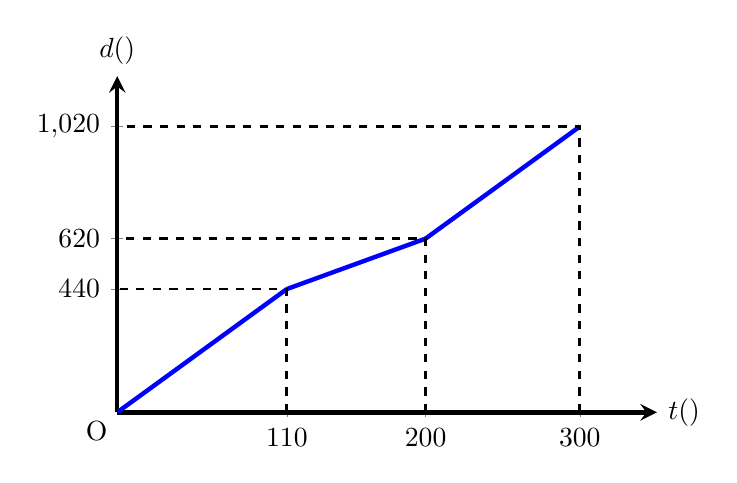
\begin{tikzpicture}  
			\begin{axis}[  ultra thick,yscale=0.75,
				xmin=0,  
				xmax=350,  
				xtick={0,110,200,300},
				ytick={0,440,620,1020},
				minor x tick num=0,
				minor y tick num=0,
				ymin=0,  
				ymax=1200, 
				samples=300,
				axis lines=center, 
				xlabel=$\xsi{t}{\left(\si{\second}\right)}$, 		ylabel=$\xsi{d}{\left(\si{\meter}\right)}$,
				every axis y label/.style={at=(current axis.above origin),anchor=south},  
				every axis x label/.style={at=(current axis.right of origin),anchor=west},  ]
				\addplot [ultra thick, blue, smooth, domain=0:110] {4*x};  
				\addplot [ultra thick, blue, smooth, domain=110:200] {440+2*(x-110)}; 
				\addplot [ultra thick, blue, smooth, domain=200:300] {620+4*(x-200)}; 
				\draw[dashed, line width=1pt] (axis cs: 110,0)--(axis cs:110,440)--(axis cs:0,440);
				\draw[dashed, line width=1pt] (axis cs: 200,0)--(axis cs:200,620)--(axis cs:0,620);
				\draw[dashed, line width=1pt] (axis cs: 300,0)--(axis cs:300,1020)--(axis cs:0,1020);
			\end{axis}  
			\node[below left] at(0,0) {O};
		\end{tikzpicture}
	\end{center}
	\choice
	{$\SI{1.2}{\meter/\second}$}
	{$\SI{1.5}{\meter/\second}$}
	{\True $\SI{2}{\meter/\second}$}
	{$\SI{2.5}{\meter/\second}$}
	\loigiai{}
\end{ex}

\Closesolutionfile{ans}
\subsection{TRẮC NGHIỆM ĐÚNG/SAI}
\setcounter{ex}{0}
\Opensolutionfile{ans}[ans/G10Y25B4-TF]
\begin{ex}
	Hai xe buýt xuất phát cùng lúc từ hai bến A và B cách nhau \SI{40}{\kilo\metre}. Xe buýt xuất phát từ A đến B với tốc độ \SI{30}{\kilo\metre/\hour} và xe buýt xuất phát từ B đến A với tốc độ \SI{20}{\kilo\metre/\hour}. Giả sử hai xe buýt chuyển động thẳng đều. Gọi $\overrightarrow{v_{12}}$ là vận tốc của xe A so với xe B, $\overrightarrow{v_{23}}$ là vận tốc của xe B so với mặt đường, $\overrightarrow{v_{13}}$ là vận tốc của xe A so với mặt đường, chọn chiều dương là chiều xe A di chuyển tới B. Nhận định tính đúng/sai của các phát biểu sau?
	\begin{center}
		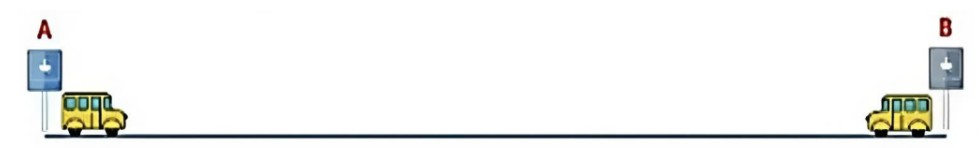
\includegraphics[scale=0.8]{figs/G10Y25B4-7}
	\end{center}
	\choiceTF[t]
	{\True Biểu thức vận tốc của xe A so với mặt đường: $v_{13} = v_{12} - v_{23}$}
	{Vận tốc của xe A so với xe B là $\SI{10}{\kilo\metre/\hour}$}
	{\True Thời gian từ lúc xuất phát đến lúc hai xe gặp nhau là $\SI{0.8}{\hour}$}
	{Quãng đường của hai xe xuất phát từ A và B đi được khi hai xe gặp nhau lần lượt là: $s_A = \SI{16}{\kilo\metre}$ và $s_B = \SI{24}{\kilo\metre}$}
	\loigiai{}
\end{ex}
\begin{ex}
	Một con tàu đang chuyển động với tốc độ $v = \SI{4}{\metre/\second}$. Một thủy thủ đang ở trên đỉnh cột buồm thì đánh rơi một ống nhòm. Trong lúc này có hai người quan sát, một người đứng trên boong tàu, một người đứng trên bờ quan sát sự việc trên.
	\choiceTF[t]
	{Ống nhòm sẽ rơi ở một vị trí phía sau cột buồm}
	{\True Người trên tàu sẽ quan sát thấy ống nhòm rơi theo phương thẳng đứng}
	{\True Người đứng trên bờ sẽ quan sát thấy ống nhòm rơi theo quỹ đạo cong hướng về phía mũi tàu}
	{Giả sử vận tốc của ống nhòm theo phương thẳng đứng khi chạm boong tàu là $u = \SI{10}{\metre/\second}$ thì vận tốc của ống nhòm so với người quan sát trên bờ là $\SI{14}{\metre/\second}$}
	\loigiai{
	\begin{itemchoice}
		\itemch Sai. Ống nhòm rơi ngay vị trí cột buồm.
		\itemch Đúng.
		\itemch Đúng.
		\itemch Sai. Vận tốc: $v'=\sqrt{v^2+u^2}\approx\SI{10.77}{\meter/\second}$.
	\end{itemchoice}
	}
\end{ex}

\begin{ex}
	Trên một xe ôtô mui trần đang chuyển động với tốc độ $v_1 = \SI{90}{\kilo\metre/\hour}$. Một người thực hiện động tác tung đồng xu, sau \SI{1}{\second} thì đồng xu trở lại tay người đó ở vị trí ban đầu. Biết rằng vận tốc của đồng xu theo phương thẳng đứng lúc vừa được tung lên có độ lớn $v_2 = \SI{5}{\metre/\second}$. Một người đứng bên đường quan sát sự việc trên.
	\choiceTF[t]
	{Đối với người bên đường tốc độ của đồng xu tại thời điểm tung là $\SI{20}{\metre/\second}$}
	{\True Khi đồng xu ở vị trí cao nhất, vận tốc của nó có phương song song với mặt đất}
	{\True Đồng xu di chuyển theo phương ngang $\SI{25}{\metre}$ kể từ khi được tung lên và hứng lại}
	{\True Người bên đường sẽ thấy quỹ đạo của đồng xu có dạng parabol}
	\loigiai{
	\begin{itemchoice}
		\itemch Sai. Vận tốc của đồng xu đối với người bên đường là $v=\sqrt{v^2_1+v^2_2}\approx\SI{25.5}{\meter/\second}$.
		\itemch Đúng.
		\itemch Đúng.
		\itemch Đúng.
	\end{itemchoice}
	}
\end{ex}
\begin{ex}
	Một sàn lan có chiều dài $\SI{60}{\metre}$ đang chuyển động ngược dòng nước. Vận tốc của sàn lan so với bờ là $\SI{2.5}{\metre/\second}$, vận tốc của nước so với bờ là $\SI{0.5}{\metre/\second}$. Một người đứng ở mũi sàn lan làm rơi một quả bóng xuống nước. Khi quả bóng trôi đến điểm giữa sàn lan thì người này mới phát hiện và đuổi theo để nhặt lại.
	\choiceTF[t]
	{Vận tốc của bóng so với bờ là $\SI{2}{\metre/\second}$}
	{\True Vận tốc của sàn lan so với nước là $\SI{3}{\metre/\second}$}
	{\True Sau khi phát hiện quả bóng người này đuổi theo với vận tốc $\SI{7}{\metre/\second}$ dọc theo sàn lan thì sẽ nhặt được quả bóng}
	{\True Vận tốc tối thiểu của người này so với sàn lan để có thể nhặt được bóng là $\SI{6}{\metre/\second}$}
	\loigiai{
	\begin{itemchoice}
		\itemch Sai. Vận tốc của bóng so với bờ là \SI{0.5}{\meter/\second}.
		\itemch Đúng.
		\itemch Đúng.\\
		\begin{itemize}
			\item Thời gian từ lúc phát hiện đến khi bóng trôi đến cuối sà lan:
			$$t_1=\dfrac{s_1}{v_{\text{b/sl}}}=\dfrac{30}{3}=\SI{10}{\second}.$$
			\item Thời gian để người di chuyển đến cuối sà lan:
			$$t_2=\dfrac{s_2}{v_{\text{n/sl}}}=\dfrac{60}{7}\approx\SI{8.57}{\second}.$$
			\item Vì $t_1>t_2$ nên người nhặt được bóng.
		\end{itemize}
		\itemch Đúng. Vận tốc tối thiểu:
		$$v_{\min}=\dfrac{s_2}{t_1}=\dfrac{60}{10}=\SI{6}{\meter/\second}.$$
	\end{itemchoice}
	}
\end{ex}


\Closesolutionfile{ans}
\subsection{TRẢ LỜI NGẮN}
\setcounter{ex}{0}
\Opensolutionfile{ans}[ans/G10Y25B4-SA]
% ===================================================================
\begin{ex}
	Một người đi xe đạp với tốc độ $v_1=\SI{5}{\meter/\second}$ bên cạnh đường ray tàu hỏa thì thấy một chiếc tàu hỏa chạy qua cùng chiều. Tốc độ của tàu hỏa là $v_2=\SI{15}{\meter/\second}$ đối với mặt đất. Sau thời gian $\SI{15}{\second}$ thì người đó thấy tàu hỏa vượt qua mặt mình. Chiều dài của tàu hỏa là bao nhiêu mét?
	\begin{center}
		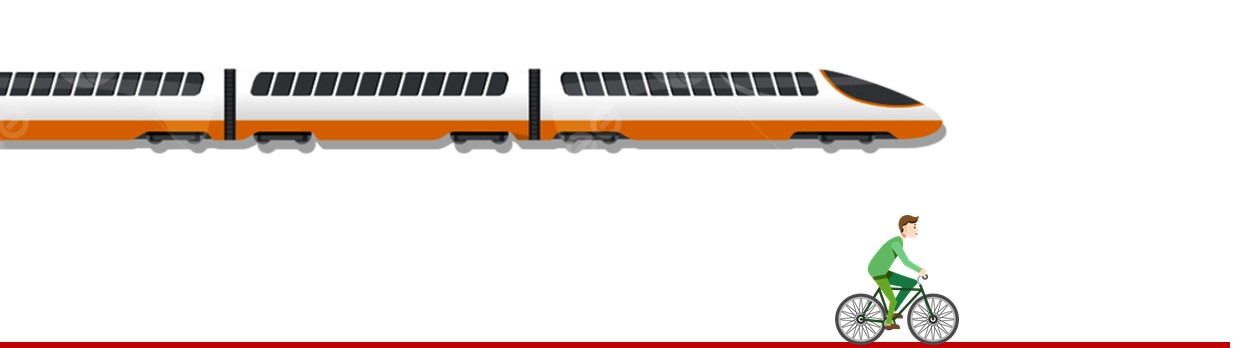
\includegraphics[scale=0.5]{figs/G10Y25B4-6}
	\end{center}
	\shortans[oly]{150}
	\loigiai{
		Vận tốc tương đối của tàu hỏa so với người:
		$$v_{21}=v_2-v_1=\SI{10}{\meter/\second}$$
		Chiều dài của tàu hỏa:
		$$L=v_{21}t=\SI{150}{\meter}.$$
	}
\end{ex}
\begin{ex}
	Hai đầu con sông A và B cách nhau \SI{6}{\kilo\meter}. Một thuyền đi từ A đến B rồi lại trở về A với tốc độ \SI{5}{\kilo\meter/\hour} khi nước đứng yên (không chảy). Thực ra nước chảy với tốc độ \SI{1}{\kilo\meter/\hour}, hãy tính thời gian chuyển động của thuyền theo đơn vị giờ.
	\shortans[oly]{2,5}
	\loigiai{
	$$t=\dfrac{s}{v_n+v_t}+\dfrac{s}{v_t-v_n}=\SI{2.5}{\hour}.$$
	}
\end{ex}

\begin{ex}
	Cứ \SI{10}{\minute} có \SI{1}{xe} buýt rời bến chuyển động thẳng đều tốc độ \SI{30}{\kilo\meter/h}. Một người đi xe đạp ngược chiều gặp \SI{2}{chiếc} xe buýt liên tiếp cách nhau \SI{7}{\minute} \SI{30}{\second}. Tìm tốc độ người đi xe đạp theo đơn vị \si{\kilo\meter/\hour}.
	\shortans[oly]{10}
	\loigiai{
	Khoảng cách giữa hai xe buýt:
	$$s=v_{\text{b/đ}}\cdot \Delta t=30\cdot\dfrac{1}{6}=\SI{5}{\kilo\meter}.$$
	Tốc độ của xe đạp đối với xe buýt:
	$$v_{\text{x/b}}=\dfrac{s}{t_{\text{x/b}}}=\dfrac{5}{1/8}=\SI{40}{\kilo\meter/\hour}.$$
	Tốc độ của xe đạp đối với đường:
	$$\vec{v}_{\text{x/đ}}=\vec{v}_{\text{x/b}}+\vec{v}_{\text{b/đ}}\Rightarrow v_{\text{x/đ}}=v_{\text{x/b}}-v_{\text{b/đ}}=\SI{10}{\kilo\meter/\hour}.$$
	}
\end{ex}

\begin{ex}
	Một máy bay đang bay theo hướng Bắc với vận tốc $\SI{200}{\meter/\second}$ thì bị gió từ hướng Tây thổi vào với vận tốc $\SI{20}{\meter/\second}$. Xác định độ lớn vận tốc tổng hợp của máy bay lúc này. Kết quả tính theo đơn vị \si{\meter/\second} và làm tròn đến chữ số hàng đơn vị.
	\loigiai{
		Gọi:
		
		$\vec v_{1,2}$ là vận tốc của máy bay so với không khí (hay so với gió, nếu coi gió là môi trường). Ở đây, $\vec v_{1,2}$ là vận tốc của máy bay theo hướng Bắc.
		$\vec v_{2,3}$ là vận tốc của gió so với mặt đất (thổi từ Tây, tức hướng sang Đông).
		$\vec v_{1,3}$ là vận tốc tổng hợp của máy bay so với mặt đất.
		
		Ta có:
		
		$$\vec v_{1,3} = \vec v_{1,2} + \vec v_{2,3}.$$
		
		Vì máy bay bay hướng Bắc và gió thổi từ Tây (hướng Đông), hai vector vận tốc này vuông góc với nhau.
		Vận tốc tổng hợp của máy bay lúc này là:
		$$v_{1,3} = \sqrt{v_{1,2}^2 + v^2_{2,3}} = \sqrt{(\SI{200}{\meter/\second})^2 + (\SI{20}{\meter/\second})^2} = \sqrt{40000+400} = \sqrt{40400} \approx \SI{201}{\meter/\second}.$$
		Vận tốc tổng hợp hướng theo hướng Đông - Bắc (nghiêng về phía Đông so với hướng Bắc). Góc hợp với hướng Bắc là $\alpha$:
		$$\tan\alpha=\dfrac{v_{23}}{v_{12}}=\dfrac{\SI{20}{\meter/\second}}{\SI{200}{\meter/\second}}=\dfrac{1}{10}\Rightarrow \alpha \approx \SI{5.7}{\degree}.$$
	}
\end{ex}

\Closesolutionfile{ans}
\subsection{TỰ LUẬN}
\setcounter{ex}{0}
\Opensolutionfile{ans}[ans/G10Y25B4-TL]
\begin{ex}
	Biết $\vec{d_1}$ là độ dịch chuyển $\SI{10}{\meter}$ về phía đông còn $\vec{d_2}$ là độ dịch chuyển $\SI{6}{\meter}$ về phía tây. Hãy xác định độ dịch chuyển tổng hợp trong 2 trường hợp sau:
	\begin{enumerate}[label=\alph*)]
		\item $\vec{d}=\vec{d_1}+\vec{d_2}$.
		\item $\vec{d}=\vec{d_1}+3\vec{d_2}$.
	\end{enumerate}
	\loigiai{
		\begin{enumerate}[label=\alph*)]
			\item Chọn chiều dương là chiều hướng đông.
			Độ dịch chuyển $\vec{d_1}$ có giá trị đại số là $\SI{10}{\meter}$.
			Độ dịch chuyển $\vec{d_2}$ có giá trị đại số là $\SI{-6}{\meter}$.
			Khi đó, độ dịch chuyển tổng hợp là:
			$d = d_1 + d_2 = \SI{10}{\meter} + (\SI{-6}{\meter}) = \SI{4}{\meter}$.
			Vậy độ dịch chuyển tổng hợp là $\SI{4}{\meter}$ về hướng đông.
			\item Chọn chiều dương là chiều hướng đông.
			Độ dịch chuyển $\vec{d_1}$ có giá trị đại số là $\SI{10}{\meter}$.
			Độ dịch chuyển $3\vec{d_2}$ có giá trị đại số là $3 \cdot (\SI{-6}{\meter}) = \SI{-18}{\meter}$.
			Khi đó, độ dịch chuyển tổng hợp là:
			$d = d_1 + 3d_2 = \SI{10}{\meter} + (\SI{-18}{\meter}) = \SI{-8}{\meter}$.
			Vậy độ dịch chuyển tổng hợp là $\SI{8}{\meter}$ về hướng tây.
		\end{enumerate}
	}
\end{ex}
\begin{ex}
	Một ô tô A chạy đều trên một đường thẳng với vận tốc $\SI{40}{\kilo\meter/\hour}$. Một ô tô B đuổi theo ô tô A với vận tốc $\SI{60}{\kilo\meter/\hour}$. Xác định vận tốc của ô tô B đối với ô tô A và của ô tô A đối với ô tô B.
	\loigiai{
		Chọn chiều dương là chiều chuyển động của hai xe.
		
		$\vec{v_\text{AD}}$ là vận tốc của xe A đối với đất;
		$\vec{v_\text{BD}}$ là vận tốc của xe B đối với đất;
		$\vec{v_\text{BA}}$ là vận tốc của xe B đối với xe A.
		
		Theo công thức cộng vận tốc:
		$$\vec{v_\text{AB}} = \vec{v_\text{AD}}+\vec{v_\text{DB}} \Rightarrow \vec{v_\text{AB}} = \vec{v_\text{AD}} - \vec{v_\text{BD}}$$
		
		Chiếu lên hướng chuyển đông của ô tô A:
		$$v_\text{AB} = \SI{40}{\kilo\meter/\hour}-\SI{60}{\kilo\meter/\hour}=\SI{-20}{\kilo\meter/\hour}$$
		
		Vậy $v_\text{BA} = \SI{20}{\kilo\meter/\hour}$.
	}
\end{ex}

\begin{ex}
	Trên đoàn tàu đang chạy thẳng với tốc độ $\SI{36}{\kilo\meter/\hour}$ so với mặt đường, một hành khách đi về đầu tàu với tốc độ $\SI{1}{\meter/\second}$ so với mặt sàn tàu.
	\begin{center}
		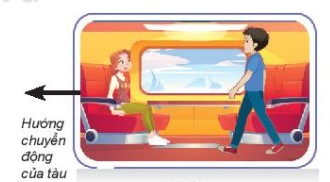
\includegraphics[scale=1]{figs/G10Y25B4-2}
	\end{center}
	\begin{enumerate}[label=\alph*)]
		\item Hành khách này tham gia mấy chuyển động?
		\item Xác định được vận tốc của hành khách đối với mặt đường.
	\end{enumerate}
	\loigiai{
		\begin{enumerate}[label=\alph*)]
			\item Hành khách này tham gia 2 chuyển động: Chuyển động với vận tốc $\SI{1}{\meter/\second}$ so với sàn tàu và chuyển động do tàu kéo đi với vận tốc bằng vận tốc của tàu so với mặt đường. Chuyển động của hành khách so với mặt đường là tổng hợp của hai chuyển động trên.
			\item Gọi:
			
			- $\vec v_{1,2}$ là vận tốc của hành khách so với tàu.
			
			- $\vec v_{2,3}$ là vận tốc của tàu so với mặt đường.
			
			- $\vec v_{1,3}$ là vận tốc của hành khách so với mặt đường.
			
			Thì:
			
			$$\vec v_{1,3} = \vec v_{1,2} + \vec v_{2,3}$$
			
			Chọn chiều chuyển động của tàu làm chiều dương:
			
			$$v_{1,3} = v_{1,2} + v_{2,3} = \SI{1}{\meter/\second} + \SI{10}{\meter/\second} = \SI{11}{\meter/\second}.$$
			
			Hướng của vận tốc người so với mặt đường là hướng đoàn tàu chạy.
		\end{enumerate}
	}
\end{ex}
\begin{ex}
	Một người bơi trong bể bơi yên lặng có thể đạt tới tốc độ $\SI{1}{\meter/\second}$. Nếu người này bơi xuôi dòng sông có dòng chảy với tốc độ $\SI{1}{\meter/\second}$ thì có thể đạt tốc độ tối đa là bao nhiêu?
	\loigiai{
		Gọi:
		
		$\vec v_{1,2}$ là vận tốc của người so với nước.
		
		$\vec v_{2,3}$ là vận tốc của nước so với bờ.
		
		$\vec v_{1,3}$ là vận tốc của người so với bờ.
		
		Ta có:
		
		$$\vec v_{1,3} = \vec v_{1,2} + \vec v_{2,3}.$$
		
		- Khi người bơi trong bể nước yên lặng, thì $v_{2,3} = \SI{0}{\meter/\second}$:
		
		$$v_{1,2} = v_{1,3} = \SI{1}{\meter/\second}.$$
		
		- Khi người này bơi xuôi dòng chảy với vận tốc $v_{2,3} = \SI{1}{\meter/\second}$:
		
		
		$$v_{1,3} = v_{1,2} + v_{2,3} = \SI{1}{\meter/\second} + \SI{1}{\meter/\second} = \SI{2}{\meter/\second}.$$
		
		Vậy nếu người này bơi xuôi dòng sông có dòng chảy với vận tốc $\SI{1}{\meter/\second}$ thì có thể đạt vận tốc tối đa là $\SI{2}{\meter/\second}.$
	}
\end{ex}
\begin{ex}
	Một ca nô chạy hết tốc lực trên mặt nước yên lặng có thể đạt $\SI{21.5}{\kilo\meter/\hour}$. Ca nô này chạy xuôi dòng sông trong $\SI{1}{\hour}$ rồi quay lại thì phải mất $\SI{2}{\hour}$ nữa mới về tới vị trí ban đầu. Hãy tính tốc độ chảy của dòng sông.
	\loigiai{
		Gọi:
		
		$\vec v_{1,2}$ là vận tốc của canô so với nước.
		
		
		$\vec v_{2,3}$ là vận tốc của nước so với bờ.
		
		
		$\vec v_{1,3}$ là vận tốc của canô so với bờ.
		
		Ta có:
		
		$$\vec v_{1,3} = \vec v_{1,2} + \vec v_{2,3}.$$
		
		- Khi canô chạy trên mặt nước yên lặng, tức $v_{2,3} = \SI{0}{\kilo\meter/\hour}$:
		
		
		$$v_{1,2} = v_{1,3} = \SI{21.5}{\kilo\meter/\hour}.$$
		
		- Khi canô chạy xuôi dòng sông, ta có:
		
		$$v_{1,3} = v_{1,2} + v_{2,3} =\dfrac{d}{t_1}$$
		
		- Khi canô quay lại, ta có:
		
		$$v'_{1,3} = v_{1,2} - v_{2,3} =\dfrac{d}{t_2}$$
		
		Thay các đại lượng của đề vào (1) và (2) ta suy ra:
		
		$$\begin{cases}
			d = \SI{28.67}{\kilo\meter}.\\
			v_{2,3} = \SI{7.17}{\kilo\meter/\hour}.
		\end{cases}$$
		
		Vậy vận tốc chảy của dòng sông là $\SI{7.17}{\kilo\meter/\hour}$.
	}
\end{ex}
\begin{ex}
	Một ca nô chạy trong hồ nước yên lặng có tốc độ tối đa $\SI{18}{\kilo\meter/\hour}$. Nếu ca nô chạy ngang một con sông có dòng chảy theo hướng Bắc - Nam với tốc độ lên tới $\SI{5}{\meter/\second}$ thì tốc độ tối đa nó có thể đạt được so với bờ sông là bao nhiêu và theo hướng nào?
	\loigiai{
		\begin{center}
			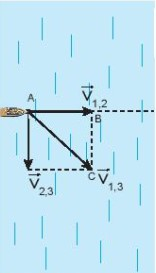
\includegraphics[scale=1]{figs/G10Y25B4-3}
		\end{center}
		Đổi: $\SI{18}{\kilo\meter/\hour} = \SI{5}{\meter/\second}$.
		Gọi vận tốc của ca nô đối với mặt nước là $\vec v_{1,2}$;
		
		Vận tốc của nước chảy đối với bờ sông là $\vec v_{2,3}$.
		
		Vận tốc của ca nô đối với bờ sông:
		
		$$\vec v_{1,3} = \vec v_{1,2} + \vec v_{2,3}.$$
		
		Vì ca nô chạy ngang sông (vuông góc với dòng chảy), nên $\vec v_{1,2}$ vuông góc với $\vec v_{2,3}$.
		Do đó, độ lớn vận tốc tổng hợp là:
		$$v_{1,3} = \sqrt{ v_{1,2}^2 + v_{2,3}^2} = \sqrt{(\SI{5}{\meter/\second})^2 + (\SI{5}{\meter/\second})^2} = \sqrt{25+25}=\sqrt{50} \approx \SI{7.07}{\meter/\second}.$$
		
		Để xác định hướng, ta có $\tan\theta = \dfrac{v_{2,3}}{v_{1,2}} = \dfrac{\SI{5}{\meter/\second}}{\SI{5}{\meter/\second}} = 1$. Suy ra $\theta = \SI{45}{\degree}$.
		Vậy vận tốc tối đa nó có thể đạt được so với bờ sông là khoảng $\SI{7.07}{\meter/\second}$ và theo hướng hợp với hướng chuyển động ngang sông một góc $\SI{45}{\degree}$ về phía xuôi dòng (hướng Đông - Nam nếu sông chảy từ Bắc xuống Nam và thuyền đi ngang từ Tây sang Đông).
	}
\end{ex}

\begin{ex}
	Một người bơi từ bờ này sang bờ kia của một con sông rộng $\SI{50}{\meter}$ theo hướng vuông góc với bờ sông. Do nước sông chảy mạnh nên quãng đường người đó bơi gấp 2 lần so với khi bơi trong bể bơi.
	\begin{enumerate}[label=\alph*)]
		\item Hãy xác định độ dịch chuyển của người này khi bơi sang bờ sông bên kia.
		\item Vị trí điểm tới cách điểm đối diện với điểm khởi hành của người bơi là bao nhiêu mét?
	\end{enumerate}
	\loigiai{
		\begin{center}
			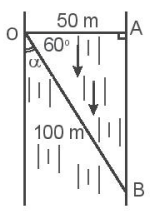
\includegraphics[scale=0.7]{figs/G10Y25B4-4}
		\end{center}
		\begin{enumerate}[label=\alph*)]
			\item $d=\text{OB}=\SI{100}{\meter}$.
			\item $\text{AB}=\text{OA}\cdot\tan\SI{60}{\degree}\approx\SI{86.7}{\meter}$.
		\end{enumerate}
	}
\end{ex}
\begin{ex}
	Một người chèo thuyền qua một con sông rộng $\SI{400}{\meter}$. Muốn cho thuyền đi theo đường AB thì người đó phải luôn hướng mũi thuyền theo hướng AC. Biết thuyền qua sông hết $\SI{8}{\minute} \SI{20}{\second}$ và tốc độ của dòng nước là $\SI{0.6}{\meter/\second}$. Tìm tốc độ của thuyền so với dòng nước.
	\begin{center}
		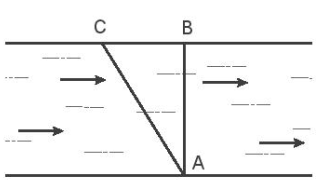
\includegraphics[scale=0.7]{figs/G10Y25B4-5}
	\end{center}
	\loigiai{
		Quãng đường nước đẩy thuyền trôi:
		$$BC=v_n\cdot t=\SI{0.6}{\meter/\second}\cdot (\SI{8}{\minute}\SI{20}{\second})=\SI{0.6}{\meter/\second}\cdot \SI{500}{\second}=\SI{300}{\meter}$$
		Tốc độ của thuyền so với dòng nước:
		$$v_\text{thuyền/nước}=\dfrac{AC}{t}=\dfrac{\sqrt{AB^2+BC^2}}{t}=\dfrac{\sqrt{(\SI{400}{\meter})^2+(\SI{300}{\meter})^2}}{\SI{500}{\second}}=\dfrac{\SI{500}{\meter}}{\SI{500}{\second}}=\SI{1}{\meter/\second}.$$
	}
\end{ex}


\begin{ex}
	Có một xe vận tốc \SI{18}{\kilo\meter/\hour} chạy trong mưa. Giả sử các giọt mưa rơi thẳng đứng và đều đối với đất.
	\begin{enumerate}[label=\alph*)]
		\item Người ngồi trên xe thấy các giọt mưa tạo góc $a = \SI{30}{\degree}$ với phương đứng. Tìm vận tốc rơi của các giọt mưa so với đất.
		\item Trên xe có một ống. Biết vận tốc rơi đều của các giọt mưa so với đất là \SI{5}{\meter/\second}. Hỏi ống phải đặt trong mặt phẳng nào, nghiêng với mặt phẳng ngang góc $a$ bằng bao nhiêu để các giọt mưa rơi thẳng đứng lọt vào ống mà không chạm thành ống.
	\end{enumerate}
	\loigiai{
	\begin{enumerate}[label=\alph*)]
		\item $v_{\text{m/đ}}\approx\SI{8.67}{\meter/\second}$.
		\item $\alpha=\SI{45}{\degree}$.
		\end{enumerate}}
\end{ex}

\begin{ex}
	Khi xuôi dòng, một canô đã vượt qua một bến ở A. Sau thời gian $t = \SI{60}{\minute}$, canô đi ngược lại và gặp bến ở C cách A \SI{6}{\kilo\meter}. Tìm tốc độ nước chảy, biết độ lớn vận tốc canô so với nước luôn không đổi và bè được thả trôi sông.
	\loigiai{
	$v_{\text{n}}=\SI{3}{\kilo\meter/\hour}$.
	}
\end{ex}



\Closesolutionfile{ans}
